At first sight the key findings discussed by Frantz and 
Kendall-Taylor hold. However, critical evaluation of a key
statistical assumption, predictive accuracy, and model 
parsimony give reason to doubt their conclusions. Following 
a brief recapitulation of the key results each point is 
briefly discussed in the remainder of this section.

\definecolor{faded}{HTML}{D9D9D9}
\definecolor{negativegrey}{HTML}{737373}
\afterpage{
\begin{figure}[!ht]
  \centering
  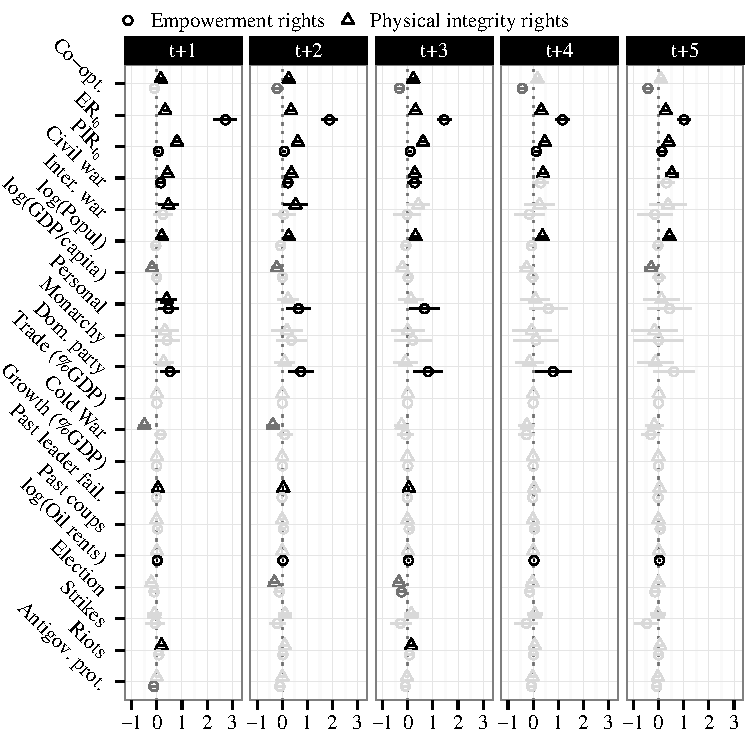
\includegraphics[width=\linewidth]{./sections/03replication/coefPlotOriginal.pdf}
  \caption{How co-optation affects political repression.
    Confidence intervals at the .95 level, 
    $\bullet$ $>0$, 
    {\color{negativegrey} $\bullet$} $<0$, 
    {\color{faded} $\bullet$} $0 \in$~CI.
    Cubic polynomials and cut points not shown.
  }
  \label{fig:coefPlot}
\end{figure}
}

Figure \ref{fig:coefPlot} summarizes all ordered logistic
regressions presented in the original article. 
Differences between the published and the replicated 
analyses are mostly negligible. With few exceptions 
coefficients and cluster robust standard errors 
agree up to two decimal places.\footnote{A fundamental
difference concerns the polynomials on tenure duration. 
The models would not converge in $R$ unless 
multicollinearity was reduced by using orthogonal 
polynomials.} As can be seen from the top row in 
Figure \ref{fig:coefPlot} higher levels of co-optation 
concur with lower levels of empowerment rights 
restrictions, but they tend to go hand in hand with 
increases in physical integrity violations. Moreover, in 
line with the idea of inert government practices the 
attenuating impact of co-optation on empowerment rights 
restrictions increases in absolute size when moving from
$t+1$ to $t+5$. The same time-dependent dynamic is not 
observable for physical integrity violations. Finally, the
models speak to the staying power of political repression 
because all lagged responses are positively signed and
statistically significant. In short, key findings can be 
reproduced and a more detailed discussion of the original 
publication is possible.

\afterpage{
\begin{table}[!htb]
\centering
\caption{Parallel-regressions assumption: $\chi^2$-comparisons}
\label{tbl:Chi2comparisons}
  \begin{tabular}{ll*{5}{c}} \toprule
    ~ & ~ & $t+1$ & $t+2$ & $t+3$ & $t+4$ & $t+5$ \\ \cmidrule{2-7}
    \multirow{2}{*}{Empowerment rights} & Unadj. P-value & 1.000 & 0.499 & 0.000 & 0.000 & 0.000 \\
    ~ & Bonf. adj. P-value & 1.000 & 0.833 & 0.000 & 0.000 & 0.000 \\
    \multirow{2}{*}{Physical integrity} & Unadj. P-value & 0.003 & 0.002 & 0.000 & 0.000 & 0.000 \\
    ~ & Bonf. adj. P-value & 0.077 & 0.052 & 0.001 & 0.000 & 0.000 \\ 
    \bottomrule
    \multicolumn{7}{l}{\textit{Note:} P-values were averaged over all imputed models.} \\
  \end{tabular}
  \end{table}
}

\begin{wrapfigure}{r}{0.45\textwidth}
\centering
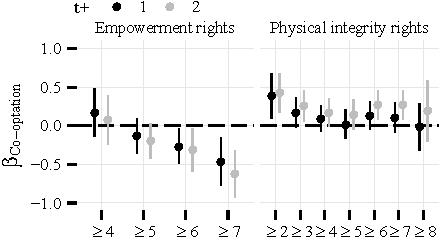
\includegraphics[width=\linewidth]{./sections/03replication/parallelRegressionsCoefPlot_manualLabels.pdf}
\caption{Separate logistic regressions}
\label{fig:separateLogisticCoef}
\end{wrapfigure}
Ordered logistic regression rests on the 
parallel-regressions assumption. It constrains differences 
between the cumulative distribution functions of any two 
categories to a constant, and thus all regression 
coefficients are assumed to be equal across categories 
\citep[476]{Fox.2008}. One way to test the assumption is a 
$\chi^2$-comparison between the constrained coefficients and 
their unconstrained alternatives from a multinomial 
regression. As shown in Table \ref{tbl:Chi2comparisons} only
the $t+1$ and $t+2$ models reject the alternative hypothesis 
of non-constant coefficients and thus support the choice of
statistical method. However, since very conservative 
Bonferroni adjusted P-values save the null an additional
inspection seems justified. To that end $j-1$ separate 
logistic regressions were fit to the set of binary responses 
$\mathbbm{1}_y(y_{i} \ge j)$.\footnote{The marginal 
categories of all responses are sparsely populated
and perfect separation occurred. The affected categories were 
discarded.} If the parallel-regressions assumption holds 
the coefficients should differ little as $j$ increases 
(c.f. \cite[107ff.]{Ward.08062014}; \cite[123]{Gelman.2006}). 
Figure \ref{fig:separateLogisticCoef} shows the results for 
the key regressor co-optation with 95 per cent confidence 
intervals added. While the right-hand panel raises little 
reason for concern, coefficients in the left-hand panel 
exhibit a clear trend. As the level of empowerment rights 
restrictions increases co-optation develops more of a punch.
In sum, the majority of models fails the 
parallel-regressions assumption, but even if it is not 
rejected further scrutiny yields reason for concern.

How well do Frantz' and Kendall-Taylor's analyses predict 
political repression in their sample? Since the consequences
of failing the parallel-regressions assumption are not well 
understood predictive accuracy might be more important than
compliance with statistical technicalities. Using separation 
plots Figure \ref{fig:sepPlot} probes this possibility for 
the four models that did not immediately fail the 
$\chi^2$-comparison \citep{Greenhill.2011}.
Their implications are unsettling. With regard to 
physical integrity violations the analyses are 
seemingly unable to discriminate between category 
members ({\color{darkgrey} $\bullet$}) and 
non-members ({\color{lightgrey} $\bullet$}). 
Furthermore, the line of predicted probabilities stays flat 
in all but the extreme categories. Turning to empowerment 
rights restrictions the state of things seems slightly 
better. Either model, $t+1$ and $t+2$, tends to predict 
higher probabilities for category members than for 
non-members. Furthermore, the line of predicted 
probabilities visibly increases across all levels of 
empowerment rights restrictions. Notwithstanding, the one-year 
lead model clearly fits the data best. In sum, decrying 
statistical significance co-optation offers little leverage 
on physical integrity violations, and only the one-year lead 
model for empowerment rights restrictions unquestionably
discriminates between members and non-members of every 
response category.

\begin{figure}[h]
  \begin{minipage}[c]{.49\linewidth}
    \centering
    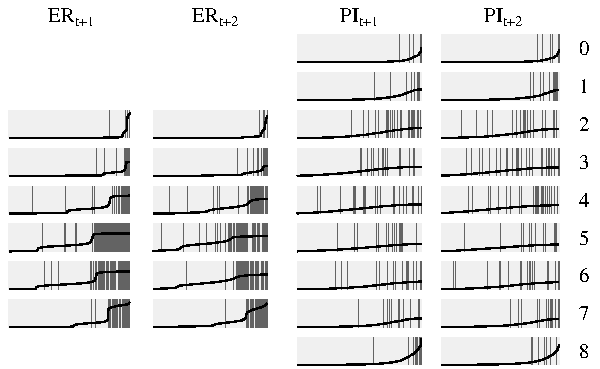
\includegraphics[width=\linewidth]{./sections/03replication/separation_revise.pdf}
    \caption{Predictive accuracy}
    \label{fig:sepPlot}
  \end{minipage}
  \hfill
  \begin{minipage}[c]{.49\linewidth}
    \centering
    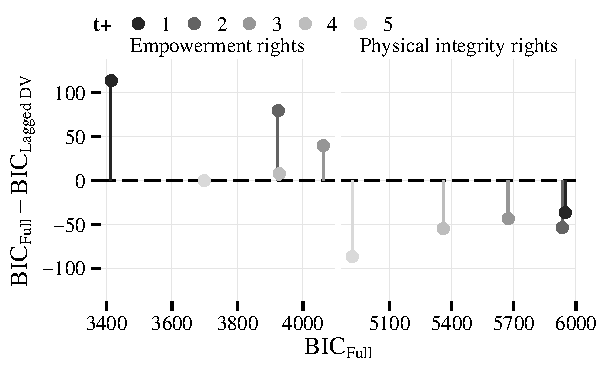
\includegraphics[width=\linewidth]{./sections/03replication/bicDifferences.pdf}
    \caption{Parsimony}
    \label{fig:bicDifferences}
  \end{minipage}
\end{figure}

However, as shown in Figure \ref{fig:coefPlot} co-optation
is not even a statistically significant predictor of
empowerment rights restrictions at $t+1$. What
variable then accounts for the separation just described? 
Figure \ref{fig:bicDifferences} probes this question. It
compares BIC values from each full model to stripped down 
versions that include only the lagged response. If the 
latter accounts for serial autocorrelation only, then 
the full set of independent variables adds explanatory 
power and the BIC should decrease. Consequently, the 
differences shown on the vertical axis of Figure 
\ref{fig:bicDifferences} should be negative.\footnote{BIC 
values were averaged over all imputations.} The results are 
again unsettling. On the one hand the differences in BICs 
for physical integrity violations are always negative and 
large in absolute value. Nonetheless, those sizeable 
improvements in model fit do not add any predictive power at
all and are thus inconsequential (c.f. Figure 
\ref{fig:sepPlot}).\footnote{Predictive accuracy declines 
with every lead. Results are available from the separation
plot scripts on my \href{https://github.com/dagtann/mleTermpaper/tree/master/R/original/onHold}{GitHub}.} On 
the other hand, differences in BIC for empowerment rights 
are always non-negative. While the one-year lead performed 
best in terms of prediction, it performs worst in terms of 
parsimony. The corresponding difference in BICs is more than
$100$ points! Hence, the improvement in fit over the 
stripped down model does not justify the inclusion of the 
full set of covariates. More generally, the single most
parsimonious predictor of empowerment rights restrictions at 
$t+1$, $t+2$, $t+3$, and $t+4$ is the lagged response. In one 
sentence: Frantz and Kendall-Taylor likely overfit their 
data.\footnote{To remove more than 20 predictors from a 
statistical model is a somewhat drastic change  and inhibits 
more nuanced assessments. Nonetheless, the results are too 
unequivocal to be mere artifacts.}

In sum, Frantz' and Kendall-Taylor's results can be 
reproduced without noteworthy deviations. However, more 
nuanced assessements show most models presented 
in the original publication fail a key statistical 
assumption of ordered logistic regression. Moreover, it 
turns out that the core findings go hand in hand with weak 
predictive accuracy and strong signs of overfitting. It is 
thus open for debate what we can learn about the 
interaction of political repression and co-optation from
Frantz' and Kendall-Taylor's analyses.